\chapter{힘, 위상 공간, 보존 법칙}

\lectureoverview{운동 법칙은 익숙한 물리량 사이의 관계를 제시하는 데 그쳐서는 안 된다. 계의 상태를 명시하고, 그 상태를 한 순간에서 다음 순간으로 옮기며, 운동 중에도 유지되는 구별과 물리량이 무엇인지 밝혀야 한다. 그럴듯하지만 틀린 힘의 법칙을 먼저 검토하고, 상태를 위치에서 위상 공간으로 확장한 뒤, 운동량과 에너지 보존을 유도하여 뉴턴 역학에 도달할 것이다.}

\section{유용한 오답 법칙}

일상적인 운동은 마찰의 영향을 크게 받는다. 무거운 물체를 바닥에서 밀면 움직이지만, 밀기를 멈추면 곧 정지한다. 일반적으로 더 큰 힘을 가하면 더 빠르게 움직이고, 더 무거운 물체를 움직이려면 더 세게 밀어야 한다. 이런 세계에서는 힘이 속도 자체를 만들어 낸다고 생각하기 쉽다. 이것이 아리스토텔레스식 운동 설명의 기본 직관이었다.

빠져 있던 경험은 빙판에서 스케이트를 타면 얻을 수 있다. 스케이터는 출발하거나 멈추거나 방향을 바꾸려면 힘이 필요하지만, 일단 움직이기 시작한 뒤 미끄러져 나아가는 데에는 힘이 필요하지 않다. 아리스토텔레스가 평범한 지면이 아니라 마찰이 거의 없는 얼음 위에서 연구했다면, 힘--속도 직관의 결함을 훨씬 알아차리기 어려웠을 것이다.

그 직관의 무엇이 잘못되었는지 드러내기 위해, 이를 현대적인 형태로 정확히 써 보자. 의도적으로 틀리게 만든 방정식을 다음과 같이 적는다.

\begin{equation}
  \mathbf F=m\mathbf v.
  \label{eq:aristotle-vector-law}
\end{equation}

이것은 뉴턴의 법칙이 아니며 물리 법칙으로 외워서는 안 된다. 이 법칙의 가치는 진단에 있다. 말로 된 규칙을 방정식으로 쓰고 나면, 그 규칙이 운동을 예측하는지, 과거를 재구성하기에 충분한 정보를 보존하는지 물을 수 있다. 힘을 뜻하는 그리스어에 관한 짧은 수업 중 토론은 \emph{dynamis}를 가리킨다. 이 어근은 dynamo나 dynamics 같은 단어에서도 찾아볼 수 있지만, 용어보다 중요한 것은 법칙 자체를 검토하는 일이다.

\begin{figure}[htbp]\centering
  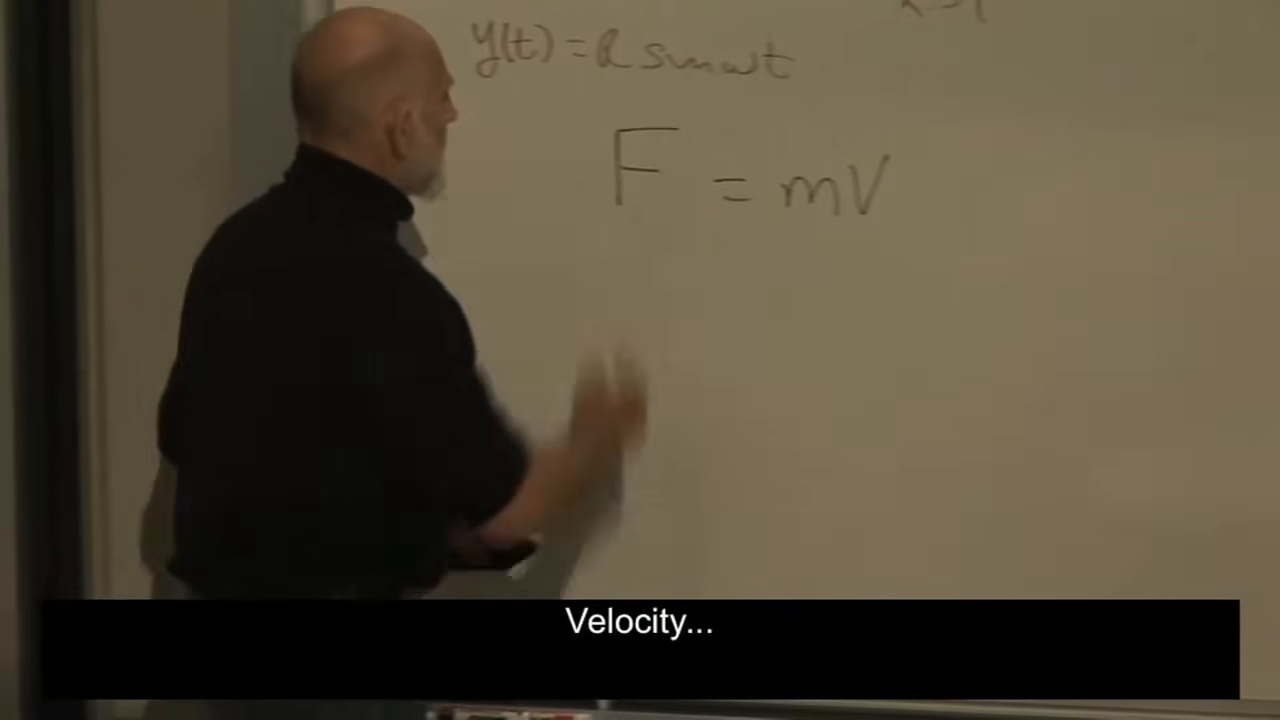
\includegraphics[width=0.82\textwidth]{lecture_02_figure_02.png}\caption{예측 가능성과 가역성을 검토하는 데 쓰는 의도적으로 틀린 힘--속도 법칙.}\lectureframe{00:04:51}\end{figure}

운동을 한 공간 좌표로 제한하자. \(v=\dot x\)이므로, 법칙은 다음과 같다.

\begin{equation}
  F(t)=m\dot x(t).
  \label{eq:aristotle-1d}
\end{equation}

이제 시간을 길이 \(\delta\)인 짧은 구간들로 나누자. 한 구간 동안에는

\begin{equation}
  \dot x(t)\simeq
  \frac{x(t+\delta)-x(t)}{\delta}.
  \label{eq:first-difference}
\end{equation}

식~\eqref{eq:aristotle-1d}에 대입하면

\begin{equation}
  x(t+\delta)
  =x(t)+\frac{\delta}{m}F(t).
  \label{eq:aristotle-update}
\end{equation}

이는 실제적인 갱신 규칙의 형태를 띤다. 현재 위치와 힘을 알면 다음 스트로보스코프 순간의 위치를 구할 수 있다. 그러나 힘이 사라지면 아리스토텔레스의 규칙은 \(\dot x=0\)을 준다. 즉, 물체는 정지 상태를 유지해야 한다. 운동을 지속시키는 힘이 없는 운동은 애초에 배제된다.

\begin{figure}[htbp]\centering
  \includegraphics[width=0.84\textwidth]{lecture_02_figure_07.png}\caption{복원력이 있을 때의 이산 아리스토텔레스 갱신. 각 단계에서 변위는 약간 1보다 작은 인자를 곱한 값이 된다.}\lectureframe{00:10:15}\end{figure}

\subsection{아리스토텔레스 역학에서의 용수철}

평형 위치가 \(x=0\)인 용수철에 연결된 입자를 생각하자. 변위가 생기면 복원력은 다음과 같다.

\begin{equation}
  F(x)=-kx,
  \qquad k>0.
  \label{eq:hooke-law}
\end{equation}

이 힘을 식~\eqref{eq:aristotle-update}에 대입하면

\begin{equation}
  x(t+\delta)
  =\left(1-\frac{k\delta}{m}\right)x(t).
  \label{eq:aristotle-spring-update}
\end{equation}

\(\delta\)가 충분히 작으면 괄호 안의 인자는 1보다 조금 작다. 따라서 매 갱신마다 변위가 같은 비율만큼 줄어든다.

\begin{equation}
  x_n=\left(1-\frac{k\delta}{m}\right)^n x_0.
  \label{eq:aristotle-geometric-decay}
\end{equation}

연속 방정식과 그 해는 다음과 같다.

\begin{align}
  m\dot x&=-kx,
  \label{eq:aristotle-spring-continuous}\\
  x(t)&=x(0)e^{-kt/m}.
  \label{eq:aristotle-spring-solution}
\end{align}

용수철은 진동하지 않는다. 어떤 변위에서 놓아도 원점에 지수적으로 가까워지며, 다가갈수록 점점 느리게 움직인다.

\begin{figure}[htbp]\centering
  \includegraphics[width=0.84\textwidth]{lecture_02_figure_08.png}\caption{아리스토텔레스식 용수철 방정식의 지수 함수 해. 변위는 진동하지 않고 감소한다.}\lectureframe{00:12:02}\end{figure}

미래를 예측하기는 쉽다. 초기 변위가 무엇이든 모두 같은 정지 상태에 가까워진다. 과거는 그렇지 않다. 입자가 유한한 정밀도로 원점 가까이에서 관측되었다고 하자. 지수적으로 작아진 흔적은 결국 모두 같은 측정 오차 범위 안에 들기 때문에, 입자는 서로 다른 여러 변위 중 어느 위치에서든 출발했을 수 있다. 수학적으로 완벽한 정밀도를 가정하면 식~\eqref{eq:aristotle-spring-solution}을 역으로 풀 수 있지만, 서로 다른 이력 사이의 실질적인 구별은 계속 지워진다. 따라서 이 법칙은 가역적인 기본 동역학이라는 관점에서 의심스럽다.

그렇다고 아리스토텔레스가 비합리적이었다는 뜻은 아니다. 그가 설명한 마찰 지배 운동은 실제로 소산적이다. 잘못은 그런 유효한 거동을 기본 법칙으로 격상한 데 있다. 마찰 자체는 복잡한 미시적 상호작용에서 생기는 힘이다. 손으로 물체를 거의 일정한 속도로 밀 때는 가한 힘이 마찰과 균형을 이룬다. 가한 힘이 속도 자체를 만들어 내는 것은 아니다.

\section{뉴턴의 법칙과 그 물리적 의미}

뉴턴 역학에서 바로잡는 핵심은 힘이 운동 상태를 변화시킨다는 것이다.

\begin{equation}
  \mathbf F=m\mathbf a=m\ddot{\mathbf x}.
  \label{eq:newton-second-law}
\end{equation}

이를 운동 방정식으로 다루기 전에, 겉보기에 순환적으로 보이는 두 가지 문제를 풀어야 한다. 첫 번째는 기준계에 관한 문제다. 뉴턴 법칙은 관성계에서 성립하고, 관성계는 뉴턴 법칙이 성립하는 기준계라고들 한다. 물리적 주장은 그런 순환 정의가 아니다. 적절한 막대자와 시계로 기술되는 \emph{실제로 존재하는} 기준계에서 뉴턴 법칙이 간단한 형태를 취한다는 경험적 주장이다. 그 기준계에 대해 가속하거나 회전하는 기준계에서는 겉보기 힘을 추가해야 한다. 그런 다른 기준계에서 방정식이 어떻게 변환되는지는 나중에 다룰 수 있다.

두 번째 순환 문제는 힘과 질량에 관한 것이다. 힘을 질량 곱하기 가속도로 정의하고 질량을 힘 나누기 가속도로 정의하면, 방정식은 아무 내용도 없는 것처럼 보인다. 조작적 실험을 하면 정의와 법칙을 구분할 수 있다. 물체를 표준 킬로그램과 저울에 걸어 비교한 뒤, 다른 힘이 없는 공간에서 그 물체를 용수철 저울에 연결한다. 용수철을 정해진 만큼 조금 늘리는 데 필요한 힘을 힘의 한 단위로 정의하자. 똑같이 늘어난 동일한 용수철 두 개는 힘 두 단위를 제공하고 가속도는 두 배로 만든다. 실제 용수철은 결국 비선형적으로 거동하거나 끊어지므로, 용수철 하나를 두 배로 늘리는 것보다 두 번째 용수철을 더하는 편이 안전하다. 용수철 하나에 같은 질량 두 개를 연결하면 가속도는 절반이 되고, 같은 질량 세 개를 연결하면 3분의 1이 된다.

\begin{figure}[htbp]\centering
  \includegraphics[width=0.84\textwidth]{lecture_02_figure_09.png}\caption{힘의 같은 단위를 정의하고 가속도가 힘에 비례하는지 검토하는 용수철 저울 사고 실험.}\lectureframe{00:22:45}\end{figure}

이 비교를 통해 다음 식에 경험적 의미가 부여된다.

\begin{equation}
  a\propto F,
  \qquad
  a\propto\frac{1}{m},
  \qquad
  F=ma.
  \label{eq:force-mass-scaling}
\end{equation}

\emph{입자}라는 말은 내부 구조가 중요하지 않은 작은 물체를 가리키는 데 쓸 것이다. 여기서 입자는 소립자에만 한정되지 않는다.

\subsection{위치만으로 상태를 나타낼 수 없는 이유}

이제 같은 스트로보스코픽 방법으로 뉴턴 방정식을 검토하자. 가속도를 나타내는 중심 유한차분은 다음과 같다.

\begin{equation}
  \ddot x(t)\simeq
  \frac{x(t+\delta)-2x(t)+x(t-\delta)}{\delta^2}.
  \label{eq:second-difference}
\end{equation}

따라서 뉴턴 방정식은 다음을 함의한다.

\begin{equation}
  x(t+\delta)
  =2x(t)-x(t-\delta)+\frac{\delta^2}{m}F(t).
  \label{eq:newton-position-update}
\end{equation}

다음 위치는 \(x(t)\)만으로 구할 수 없다. 이전 위치 \(x(t-\delta)\), 또는 이에 동등하게 현재 순간의 속도도 알아야 한다. 처음에는 이 때문에 뉴턴 방정식이 아리스토텔레스 법칙보다 예측력이 떨어지는 것처럼 보인다. 그러나 올바른 결론은 위치만으로는 상태를 완전히 기술할 수 없다는 것이다. 어떤 한 순간에 관련된 정보를 모두 안다는 것은 이후 운동을 결정하기에 충분한 자료를 안다는 뜻이다. 뉴턴 입자에서는 위치와 속도가 그 자료에 해당한다.

\section{운동량과 위상 공간}

운동량을 다음과 같이 도입하자.

\begin{equation}
  \mathbf p=m\mathbf v=m\dot{\mathbf x}.
  \label{eq:momentum-definition}
\end{equation}

고정된 뉴턴 계의 질량은 일정하다고 가정한다. 물체의 일부가 떨어져 나갈 수는 있다. 예컨대 펜에서 뚜껑이 떨어져 나갈 수 있지만, 그러면 기술 대상인 물체가 달라진 것이다. 선택한 닫힌 계의 전체 질량은 여전히 일정하다. \(m\)가 일정하면 뉴턴의 제2법칙은 다음과 같이 된다.

\begin{equation}
  \mathbf F=\dot{\mathbf p}.
  \label{eq:newton-momentum-form}
\end{equation}

\begin{figure}[htbp]\centering
  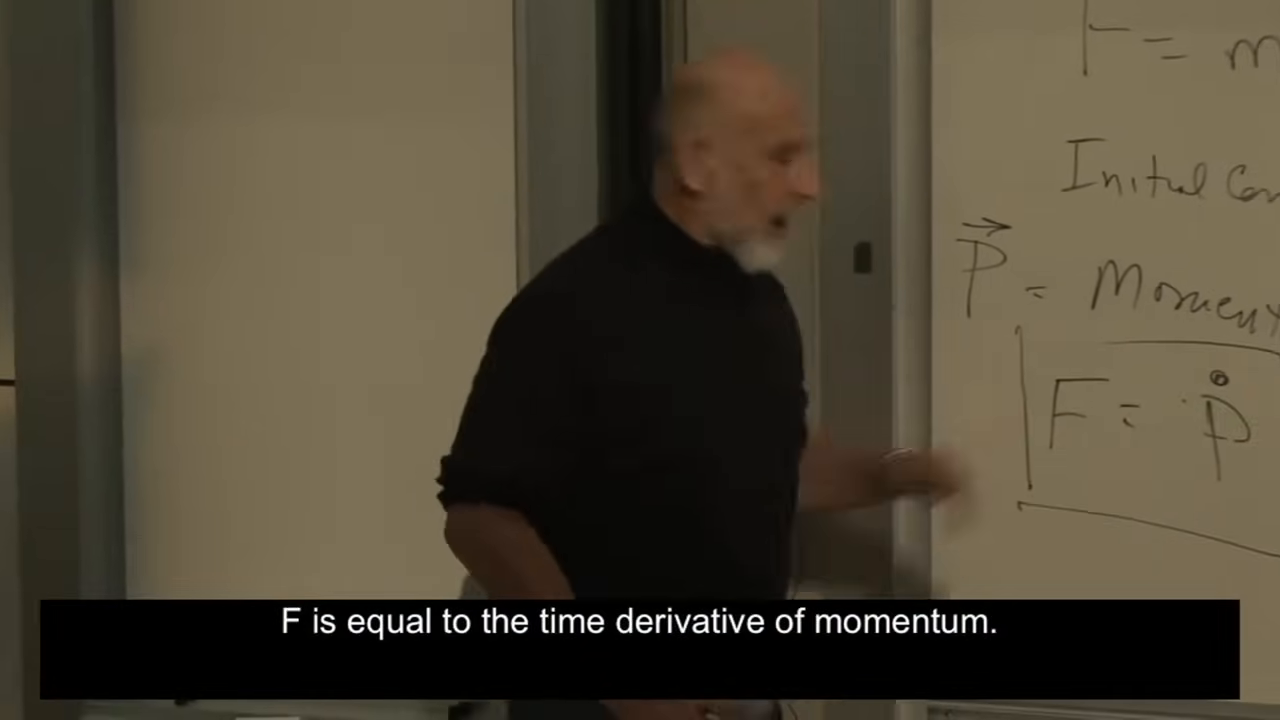
\includegraphics[width=0.82\textwidth]{lecture_02_figure_03.png}\caption{운동량의 시간 미분으로 나타낸 뉴턴의 법칙.}\lectureframe{00:32:35}\end{figure}

한 좌표에서 뉴턴 운동은 서로 독립적인 상태 변수 두 개에 관한 1계 방정식 두 개로 쓸 수 있다.

\begin{align}
  \dot p&=F(x,t),
  \label{eq:first-order-p}\\
  \dot x&=\frac{p}{m}.
  \label{eq:first-order-x}
\end{align}

한 방정식은 힘이 운동량을 어떻게 변화시키는지 말하고, 다른 방정식은 운동량이 위치를 어떻게 변화시키는지 말한다. 이에 대응하는 이산 1계 형태는 다음과 같다.

\begin{align}
  p(t+\delta)&=p(t)+\delta F(x(t),t)+O(\delta^2),
  \label{eq:momentum-discrete}\\
  x(t+\delta)&=x(t)+\frac{\delta}{m}p(t)+O(\delta^2).
  \label{eq:position-discrete}
\end{align}

\(x(t)\)와 \(p(t)\)를 알면, 이 방정식들로 다음 순간의 두 값을 구할 수 있다. 그 값들이 다음 단계의 입력이 된다. 이렇게 갱신을 반복해 궤적을 만든다.

\begin{figure}[htbp]\centering
  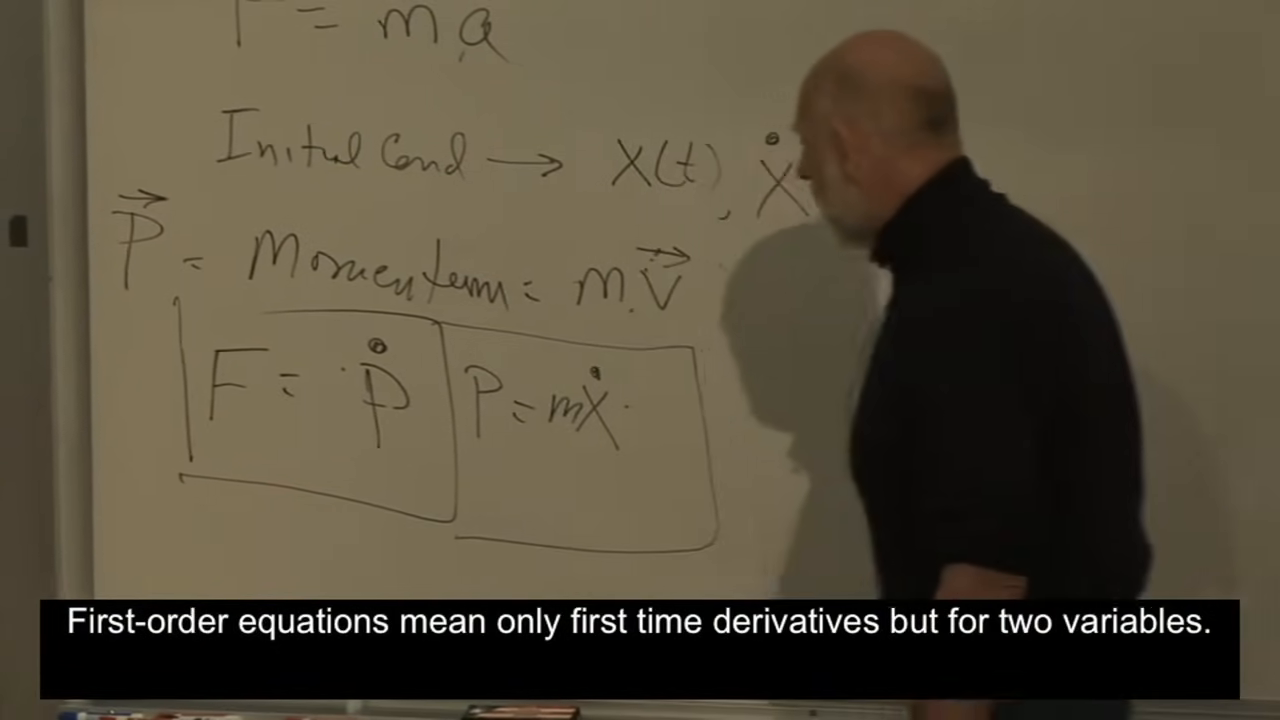
\includegraphics[width=0.84\textwidth]{lecture_02_figure_04.png}\caption{두 개의 1계 방정식과 그에 대응하는 초기 자료. 위치와 운동량을 함께 주면 상태가 정해진다.}\lectureframe{00:35:47}\end{figure}

모든 순서쌍 \((x,p)\)이 이루는 공간을 \emph{위상 공간}이라 한다. 3차원에서 움직이는 입자 하나의 위상 공간은 좌표 여섯 개로 이루어진다.

\begin{equation}
  (x,y,z,p_x,p_y,p_z).
  \label{eq:one-particle-phase-space}
\end{equation}

위상 공간은 완전한 초기 조건들의 공간이다. 배치 공간은 위치만 기록하지만, 위상 공간은 운동 법칙에 필요한 자료를 정확히 기록한다.

\begin{classroomqa}\audiencequestion{힘이 시간에 따라 주어지는 함수가 아니라 위치의 함수라면, 갱신이 더 복잡해지나요?\lecturetimestamp{00:36:27--00:37:07}}\lecturerresponse{방정식은 여전히 운동을 예측한다. \(x\)와 \(p\)를 알면 \(F(x)\)의 값을 안다. 식~\eqref{eq:first-order-p}은 \(p\)를 갱신하고, 식~\eqref{eq:first-order-x}은 \(x\)를 갱신하므로, 갱신된 순서쌍을 다시 사용할 수 있다.}\end{classroomqa}

\section{뉴턴 역학의 용수철}

두 법칙을 같은 물리적 조건에서 비교하기 위해 용수철로 돌아가자. 뉴턴 법칙은 다음과 같다.

\begin{equation}
  m\ddot x=-kx.
  \label{eq:newton-spring}
\end{equation}

상수를 없애기 위해 잠시 \(m=k=1\)로 놓자. 그러면

\begin{equation}
  \ddot x=-x.
  \label{eq:normalized-oscillator}
\end{equation}

지수 함수와 달리 사인과 코사인은 두 번 미분하면 자기 자신에 음수를 곱한 함수가 된다. 일반해는 다음과 같이 쓸 수 있다.

\begin{align}
  x(t)&=C\cos(t-t_0),
  \label{eq:oscillator-x}\\
  p(t)=\dot x(t)&=-C\sin(t-t_0).
  \label{eq:oscillator-p}
\end{align}

두 상수에는 초기 정보 두 가지가 담겨 있다. 진폭 \(C\)은 최대 변위를 나타내고, \(t_0\)은 위상을 정한다. 여기서는 \(t=t_0\)에서 속도가 영이 되도록 위상을 정했다. 입자는 양 끝점에서 순간적으로만 멈춘다. 그런 다음 되돌아와 원점을 지나며, 그곳에서 속력과 운동량이 최대가 되고 계속 진동한다.

식~\eqref{eq:oscillator-x}과 \eqref{eq:oscillator-p}의 양변을 제곱하면 다음과 같다.

\begin{equation}
  x^2+p^2=C^2.
  \label{eq:oscillator-phase-circle}
\end{equation}

따라서 위상 공간의 점은 반지름이 \(C\)인 원을 따라 움직인다. 초기 진폭이 다르면 서로 다른 원이 생기고, \(t_0\)을 바꾸면 같은 원 위에서 출발점이 달라진다. 모든 원은 진폭과 관계없이 이 정규화된 단위계에서 같은 주기 \(2\pi\)로 한 바퀴를 돈다.

\begin{figure}[htbp]\centering
  \includegraphics[width=0.84\textwidth]{lecture_02_figure_10.png}\caption{진동자의 해와 \((x,p)\) 위상 평면에서의 원 궤도.}\lectureframe{00:43:20}\end{figure}

\begin{figure}[htbp]\centering
  \begin{tikzpicture}[scale=1.05,>=Latex]
    \draw[->] (-2.6,0) -- (2.75,0) node[right] {$x$};
    \draw[->] (0,-2.4) -- (0,2.55) node[above] {$p$};
    \draw[blue!65!black,thick] (0,0) circle (1.85);
    \draw[->,blue!65!black,thick]
      (1.60,0.93) arc[start angle=30,end angle=72,radius=1.85];
    \fill[red!65!black] (1.60,0.93) circle (2pt);
    \draw[dashed] (0,0) -- (1.60,0.93)
      node[midway,below right] {$C$};
    \node[align=left] at (-1.55,1.85)
      {$x=C\cos(t-t_0)$\\$p=-C\sin(t-t_0)$};
  \end{tikzpicture}\caption{위상 공간의 궤도에는 위치와 운동량이 모두 담겨 있다. 반지름은 운동을 구별하고, 각도는 시간에 따라 일정한 속도로 증가한다.}\label{fig:oscillator-phase-space}\end{figure}

수평축에 사영하면 \(x\)의 익숙한 왕복 운동이 나타나고, 수직축에 사영하면 \(p\)의 진동이 나타난다. 아리스토텔레스식 용수철과 달리 서로 다른 원은 합쳐지지 않는다. 위상 공간의 한 점을 알면 미래와 과거를 모두 결정할 수 있다.

일반적인 \(m\)와 \(k\)의 경우 각진동수는 다음과 같다.

\begin{equation}
  \omega=\sqrt{\frac{k}{m}},
  \qquad
  x(t)=C\cos\bigl(\omega(t-t_0)\bigr),
  \label{eq:general-oscillator-frequency}
\end{equation}

그러면 위상 공간 궤도는 축의 눈금을 조정하지 않은 \((x,p)\) 평면에서 타원이 된다. 원으로 나타낸 그림은 강의에서 사용한 편리한 \(m=k=1\) 정규화에 따른 것이다.

\begin{classroomqa}\audiencequestion{진동자 방정식의 2계 미분을 1계 미분으로 바꾸면 예측 가능성을 잃게 되나요?\lecturetimestamp{00:45:23--00:46:04}}\lecturerresponse{아니요. 적절한 초기 자료가 주어지면 1계 방정식도 미래의 운동을 예측할 수 있습니다. 더 근본적인 쟁점은 그 흐름이 가역성을 유지할 만큼 충분히 구별을 보존하는지 여부입니다. 이에 관한 일반 정리는 필요한 수학적 도구를 갖춘 뒤에 다루겠습니다.}\end{classroomqa}

\section{시간 반전}

진동자의 그림은 가역성을 구체적으로 보여 주지만, 방정식에 직접 적용해 검토할 수도 있다. 반전된 시간 좌표를 도입하자.

\begin{equation}
  T=-t.
  \label{eq:reverse-time}
\end{equation}

그러면

\begin{equation}
  \frac{d}{dt}=-\frac{d}{dT},
  \qquad
  \frac{d^2}{dt^2}=\frac{d^2}{dT^2}.
  \label{eq:time-derivative-parity}
\end{equation}

시간 반전에서 1계 미분은 부호가 바뀌지만 2계 미분은 그렇지 않다. 따라서 자율적인 아리스토텔레스 방정식

\begin{equation}
  m\dot x=F(x)
  \label{eq:aristotle-time-reversal}
\end{equation}

은 영화를 거꾸로 재생해도 같은 형태를 유지하지 않는다. 감쇠하는 용수철은 평형점에서 저절로 멀어지는 용수철로 바뀔 것이다. 반면에

\begin{equation}
  m\ddot x=F(x)
  \label{eq:newton-time-reversal}
\end{equation}

은 변하지 않는다. 뉴턴 역학의 영화를 거꾸로 재생하면 속도는 반전되지만 가속도는 그대로이므로, 역방향 영화도 허용되는 해가 된다.

\begin{figure}[htbp]\centering
  \includegraphics[width=0.84\textwidth]{lecture_02_figure_11.png}\caption{\(t\mapsto -t\)에서의 칠판 비교. 1계 미분은 부호가 반전되지만 2계 미분은 그렇지 않다.}\lectureframe{00:50:45}\end{figure}

\begin{classroomqa}\audiencequestion{가역성을 물리학 일반의 전제로 받아들여야 하는 이유는 무엇인가요?\lecturetimestamp{00:46:16--00:48:26}}\lecturerresponse{가역성은 정의상 보장되는 것이 아니라 실험으로 검증된다. 성공적인 법칙을 살펴보고 공통된 실험적 특징을 찾아 그 특징을 원리로 끌어올린다. 더 깊은 논리적 순서는 반대 방향으로 진행된다. 양자장론이 더 근본적이며, 뉴턴 역학은 느린 운동이나 큰 물체와 같은 근사를 통해 나타난다. 하지만 강의에서는 더 단순한 법칙에서 출발해 단계적으로 쌓아 올려야 한다. 따라서 지금 가역성을 원리로 도입하고, 그 원리가 어디까지 적용되는지는 나중에 검토할 것이다.}\end{classroomqa}

\begin{classroomqa}\audiencequestion{뉴턴은 가역성 자체를 의식적으로 문제로 여겼나요?\lecturetimestamp{00:48:28--00:49:02}}\lecturerresponse{역사적으로는 확실하지 않다. 뉴턴은 관성을 분명히 이해했다. 즉, 등속 운동을 유지하는 데 힘이 필요한 것이 아니라 운동 상태를 바꾸는 데 힘이 필요하다는 점을 이해했다. 그 통찰을 가역성이라는 관점에서 명시적으로 정식화했는지는 별개의 역사적 문제다.}\end{classroomqa}

\section{주기 운동과 보존량}

위상 공간의 원에서 다음 발상을 얻을 수 있다. 궤적은 하나의 원 위에 머물며 다른 원으로 뛰어넘지 않는다. 따라서 운동 내내 일정하게 유지되는 수로 원을 표시할 수 있다. 정규화된 진동자에서 그 수는 다음과 같다.

\begin{equation}
  C^2=x^2+p^2.
  \label{eq:cycle-label}
\end{equation}

절반에 해당하는 계수를 제외하면 이것은 진동자의 에너지다. 원이 클수록 에너지가 크며, 시작 위상을 바꾸어도 에너지는 변하지 않는다. 이 진술을 그림에서 읽어내는 데 그치지 않고 유도하겠지만, 먼저 운동량을 살펴보자.

뉴턴의 제1법칙에 따르면 알짜힘을 받지 않는 물체는 일정한 속도로 움직인다. 이 법칙은 이미 제2법칙에 포함되어 있다.

\begin{equation}
  \mathbf F=0
  \quad\Longrightarrow\quad
  \dot{\mathbf p}=0
  \quad\Longrightarrow\quad
  \mathbf v=\text{constant}
  \label{eq:newton-first-from-second}
\end{equation}

질량이 일정한 경우에 그렇다. 뉴턴의 제3법칙은 입자 사이의 상호작용에 관한 새로운 정보를 제공한다.

\subsection{같은 크기와 반대 방향의 힘, 그리고 중심력}

\(\mathbf F_{ij}\)는 입자 \(i\)에 입자 \(j\)가 가하는 힘을 나타낸다. 제3법칙의 작용·반작용 부분은 다음과 같다.

\begin{equation}
  \mathbf F_{ij}=-\mathbf F_{ji}.
  \label{eq:newton-third-pair}
\end{equation}

두 힘이 같은 방향을 가리킨다면, 고립된 두 입자 쌍이 저절로 가속할 수 있을 것이다. 내부 힘만으로 운동을 만들어 내는 추진제 없는 기계가 되는 셈이다. 그런 거동은 관측되지 않는다.

\begin{figure}[htbp]\centering
  \includegraphics[width=0.84\textwidth]{lecture_02_figure_12.png}\caption{작용과 반작용의 힘을 첨자로 표시한 식.}\lectureframe{00:59:25}\end{figure}

여기서 다루는 점입자 힘의 경우 두 힘은 입자 중심을 잇는 직선을 따라 작용하기도 한다. 서로 크기가 같고 방향이 반대지만 한 직선 위에 놓이지 않는 힘은 순수한 토크를 이루어 고립된 강체 두 입자 쌍을 회전시킬 수 있다. 중심력 조건은 이를 막는다.

\begin{equation}
  \mathbf F_{ij}\parallel
  (\mathbf r_i-\mathbf r_j).
  \label{eq:central-force-condition}
\end{equation}

작용·반작용 조건으로 선운동량 보존을 얻을 수 있다. 두 입자를 잇는 직선 위에서 작용한다는 조건은 나중에 다룰 각운동량 보존과 관련된다.

\begin{figure}[htbp]\centering
  \includegraphics[width=0.84\textwidth]{lecture_02_figure_13.png}\caption{뉴턴 제3법칙의 중심력 조건. 상호작용 힘은 두 입자를 잇는 직선을 따라 작용한다.}\lectureframe{01:01:38}\end{figure}

\subsection{전체 운동량}

\(N\)개의 입자로 된 닫힌 계를 생각하자. 외부에서 작용하는 힘은 없고, 입자들이 서로에게 가하는 힘만 존재한다. 힘의 가산성과 뉴턴의 제2법칙에 따라 각 입자에 대해 다음이 성립한다.

\begin{equation}
  \dot{\mathbf p}_i
  =m_i\ddot{\mathbf r}_i
  =\sum_{\substack{j=1\\j\ne i}}^N \mathbf F_{ij}.
  \label{eq:many-particle-newton}
\end{equation}

이 식을 \(i\)에 대해 합하면

\begin{align}
  \frac{d}{dt}\sum_{i=1}^N\mathbf p_i
  &=\sum_{i=1}^N
    \sum_{\substack{j=1\\j\ne i}}^N\mathbf F_{ij}
  \notag\\
  &=\sum_{i<j}\bigl(\mathbf F_{ij}+\mathbf F_{ji}\bigr)
  =0.
  \label{eq:momentum-pair-cancellation}
\end{align}

모든 상호작용은 양쪽 방향으로 한 번씩 나타나며, 두 힘은 서로 상쇄된다. 다음과 같이 정의하면

\begin{equation}
  \mathbf P_{\mathrm{tot}}=\sum_{i=1}^N\mathbf p_i,
  \label{eq:total-momentum}
\end{equation}

첫 번째 보존 법칙을 얻는다.

\begin{equation}
  \frac{d\mathbf P_{\mathrm{tot}}}{dt}=0.
  \label{eq:momentum-conservation}
\end{equation}

\begin{figure}[htbp]\centering
  \includegraphics[width=0.84\textwidth]{lecture_02_figure_14.png}\caption{입자별 방정식을 합하면 쌍을 이루는 힘들이 상쇄되고, 전체 운동량의 미분은 0이 된다.}\lectureframe{01:04:38}\end{figure}

역사적으로는 운동량 보존을 뉴턴 제3법칙의 결과로 설명해 왔다. 현대 물리학에서는 운동량 보존을 더 근본적인 진술로 보는 경우가 많다. 고립된 두 입자 계에서 전체 운동량이 보존된다면, 내부 운동량의 변화는 크기가 같고 방향이 반대여야 한다. 그러나 지금의 전개에서는 뉴턴 역학을 통한 설명이 유용하다.

\section{1차원에서의 에너지}

위치에만 의존하는 힘을 받아 직선 위를 움직이는 입자 하나를 생각하자.

\begin{equation}
  F=F(x).
  \label{eq:position-force}
\end{equation}

이런 힘을 시간 독립적이라고 한다. 움직이는 입자가 받는 힘의 수치가 일정하다는 뜻은 아니다. 그 값은 \(x(t)\)가 변함에 따라 달라진다. 입자가 같은 위치 \(x\)에 있을 때에는 시계가 가리키는 시간과 관계없이 같은 힘을 받는다는 뜻이다.

1차원에서는 충분히 매끄러운 힘 함수를 적분할 수 있다. 따라서 위치 에너지 \(V(x)\)를 다음과 같이 정의하자.

\begin{equation}
  F(x)=-\frac{dV}{dx},
  \label{eq:potential-definition-1d}
\end{equation}

또는 다음과 같이 쓸 수 있다.

\begin{equation}
  V(x)=-\int^x F(u)\,du+V_0.
  \label{eq:potential-integral}
\end{equation}

덧셈 상수 \(V_0\)는 힘에 영향을 주지 않는다. \(V(x)\)을 \(x\)축 위에 놓인 지형의 높이라고 생각해 보자. 입자는 높이가 낮아지는 쪽으로 밀리며, 기울기가 가파를수록 힘이 크다. 매끄러운 언덕의 꼭대기나 바닥에서는 기울기가 영이므로 그곳의 힘도 사라진다.

\begin{figure}[htbp]\centering
  \includegraphics[width=0.84\textwidth]{lecture_02_figure_15.png}\caption{1차원 지형으로 나타낸 위치 에너지. 힘은 내리막 방향을 향하고 그 크기는 기울기에 따라 정해진다.}\lectureframe{01:12:57}\end{figure}

운동 에너지, 위치 에너지, 전체 에너지를 다음과 같이 정의하자.

\begin{equation}
  T=\frac12m\dot x^2,
  \qquad
  E=T+V(x)
  =\frac12m\dot x^2+V(x).
  \label{eq:energy-1d}
\end{equation}

이 단계에서 에너지는 보존 후보량에 붙인 이름일 뿐이다. 지형 그림은 그 물리적 의미를 보여 준다. 내리막을 구르면 \(V\)가 낮아지는 동시에 속도가 커지므로 \(T\)가 증가하고, 오르막을 올라갈 때에는 반대가 된다. 뉴턴 방정식으로 두 에너지의 교환이 정확히 일어난다는 것을 증명할 수 있다.

식~\eqref{eq:energy-1d}을 미분하자. \(m\)는 상수이고 \(V\)는 \(x(t)\)를 통해서만 시간에 의존하므로

\begin{align}
  \frac{dE}{dt}
  &=m\dot x\ddot x+\frac{dV}{dx}\dot x
  \notag\\
  &=\dot x\left(m\ddot x+\frac{dV}{dx}\right).
  \label{eq:energy-derivative-1d}
\end{align}

뉴턴의 법칙과 \(V\)의 정의에 따르면

\begin{equation}
  m\ddot x=F=-\frac{dV}{dx}.
  \label{eq:newton-potential-1d}
\end{equation}

따라서 식~\eqref{eq:energy-derivative-1d}의 대괄호 안 항은 영이 된다:

\begin{equation}
  \frac{dE}{dt}=0.
  \label{eq:energy-conservation-1d}
\end{equation}

\begin{figure}[htbp]\centering
  \includegraphics[width=0.84\textwidth]{lecture_02_figure_16.png}\caption{1차원 에너지의 시간 미분을 속도와 뉴턴 방정식의 곱으로 인수분해한 식.}\lectureframe{01:19:18}\end{figure}

1차원에서는 위치에 의존하는 힘이 충분히 매끄럽기만 하면 그 힘의 부정적분이 존재하므로, 이 조건 외에 추가적인 동역학적 가정은 필요하지 않았다.

\section{여러 차원과 보존력}

좌표가 \(x_i\)인 입자 하나에 대해 뉴턴 방정식의 각 성분은 다음과 같다.

\begin{equation}
  F_i(\mathbf x)=m\ddot x_i.
  \label{eq:newton-components}
\end{equation}

힘의 성분 \(F_i\)은 \(x_i\)에만 의존하는 것이 아니라 모든 좌표에 의존할 수 있다. 다음 조건을 만족하는 스칼라 함수 하나 \(V(\mathbf x)\)를 찾고자 한다.

\begin{equation}
  F_i(\mathbf x)
  =-\frac{\partial V(\mathbf x)}{\partial x_i},
  \qquad
  \mathbf F=-\boldsymbol\nabla V.
  \label{eq:gradient-force}
\end{equation}

1차원에서의 구성과 달리, 이것이 자동으로 가능하지는 않다. 일반적으로 임의의 세 함수 \(F_1,F_2,F_3\)에는 스칼라 함수 하나의 미분에 담을 수 있는 것보다 독립적인 정보가 더 많이 들어 있다. 달리 말해, 힘장이 잠재함수에서 나오려면 적절한 혼합 편미분의 일치와 같은 호환 조건을 만족해야 한다. 단일 연결 영역에서는 이를 \(\boldsymbol\nabla\times\mathbf F=0\)로 나타낸다. 따라서 식~\eqref{eq:gradient-force}는 수학적 항등식이 아니라 여기서 다루는 힘의 종류에 대한 물리적 가정으로 둔다.

\begin{figure}[htbp]\centering
  \includegraphics[width=0.84\textwidth]{lecture_02_figure_17.png}\caption{다차원 힘의 법칙과 위치 에너지의 등고선 그림. 힘은 등고선을 가로질러 \(V\)가 감소하는 방향을 향한다.}\lectureframe{01:24:15}\end{figure}

등고선 지도에서 \(V\)는 각 등고선을 따라 일정하다. 그래디언트는 등고선에 수직이며 가장 가파르게 증가하는 방향을 가리킨다. 힘 \(-\boldsymbol\nabla V\)는 가장 가파르게 감소하는 방향을 가리킨다.

\begin{figure}[htbp]\centering
  \begin{tikzpicture}[scale=1.0,>=Latex]
    \draw[->] (-3.0,0) -- (3.1,0) node[right] {$x_1$};
    \draw[->] (0,-2.4) -- (0,2.55) node[above] {$x_2$};
    \draw[orange!65!black,thick]
      plot[smooth cycle] coordinates
      {(-0.55,-0.35) (0.15,-0.55) (0.72,-0.10) (0.50,0.53) (-0.25,0.65)};
    \draw[orange!65!black,thick]
      plot[smooth cycle] coordinates
      {(-1.15,-0.75) (0.20,-1.10) (1.35,-0.25) (1.10,0.95) (-0.45,1.25)};
    \draw[orange!65!black,thick]
      plot[smooth cycle] coordinates
      {(-1.85,-1.20) (0.15,-1.70) (2.15,-0.40) (1.70,1.50) (-0.80,1.85)};
    \draw[->,blue!65!black,very thick] (1.62,0.73) -- (0.82,0.20)
      node[midway,above left] {$\mathbf F$};
    \draw[dashed,->,red!65!black,thick] (0.82,0.20) -- (1.62,0.73)
      node[midway,below right] {$\boldsymbol\nabla V$};
    \node[orange!65!black] at (-1.62,1.45) {$V=V_3$};
    \node[orange!65!black] at (-0.92,0.92) {$V=V_2$};
    \node[orange!65!black] at (-0.35,0.30) {$V=V_1$};
  \end{tikzpicture}\caption{스칼라 위치 에너지의 등고선. 그래디언트는 등고선의 법선 방향이며, 보존력은 그 반대 방향을 향한다.}\label{fig:potential-contours}\end{figure}

식~\eqref{eq:gradient-force}이 성립할 때 다음과 같이 정의하자.

\begin{equation}
  E=\frac12m\sum_i\dot x_i^2+V(x_1,\ldots,x_n).
  \label{eq:energy-many-coordinates}
\end{equation}

운동에너지 항은 질량에 속도 벡터의 크기 제곱을 곱한 값의 절반이다. 이를 미분하고 다변수 연쇄 법칙을 적용하면 다음을 얻는다.

\begin{align}
  \frac{dE}{dt}
  &=m\sum_i\dot x_i\ddot x_i
    +\sum_i\frac{\partial V}{\partial x_i}\dot x_i
  \notag\\
  &=\sum_i\dot x_i
    \left(m\ddot x_i+\frac{\partial V}{\partial x_i}\right)
  =0.
  \label{eq:energy-derivative-multidimensional}
\end{align}

증명은 첨자를 붙인 것만 빼면 1차원 증명과 정확히 같다. 다만 그 전제가 더 강하다. 모든 힘의 성분이 하나의 위치 에너지 함수에서 나와야 한다.

\begin{figure}[htbp]\centering
  \includegraphics[width=0.84\textwidth]{lecture_02_figure_18.png}\caption{첨자가 붙은 에너지 미분. 각 대괄호 안 항은 뉴턴 방정식의 해당 성분에 따라 사라진다.}\lectureframe{01:28:30}\end{figure}

3차원에서 \(N\)개의 입자를 생각하고, 모든 좌표를 하나의 목록으로 모으면 다음과 같다.

\begin{equation}
  \begin{aligned}
    q_a={}&(x_1,y_1,z_1,x_2,y_2,z_2,\ldots,\\[-0.2em]
           &\phantom{(}x_N,y_N,z_N),\\
    &a=1,\ldots,3N.
  \end{aligned}
  \label{eq:flattened-coordinates}
\end{equation}

좌표 항은 \(3N\)개지만 입자의 질량은 \(N\)개다. 각 입자에 속하는 세 좌표 항에는 같은 질량이 들어간다. 만약

\begin{equation}
  F_a=-\frac{\partial V(q_1,\ldots,q_{3N})}{\partial q_a},
  \label{eq:many-particle-conservative-force}
\end{equation}

이라면

\begin{equation}
  E=\sum_{A=1}^{N}\frac12m_A\lvert\dot{\mathbf r}_A\rvert^2
    +V(\mathbf r_1,\ldots,\mathbf r_N)
  \label{eq:many-particle-energy}
\end{equation}

같은 계산에 따라 보존된다. 위치 에너지에서 나오는 힘을 \emph{보존력}이라고 부르는 까닭은 바로 이 보존 법칙이 성립하기 때문이다. 여기서 보존력이라는 말은 정치적인 뜻이 없다.

\section{에너지 등고선으로 본 진동자}\enlargethispage{3\baselineskip}

용수철 힘 \(F=-kx\)에 대해 식~\eqref{eq:potential-definition-1d}는 다음을 준다.

\begin{equation}
  V(x)=\frac12kx^2+V_0.
  \label{eq:spring-potential}
\end{equation}

\(V_0=0\)로 정하면 진동자의 에너지는 다음과 같다.

\begin{equation}
  E=\frac12m\dot x^2+\frac12kx^2
   =\frac{p^2}{2m}+\frac12kx^2.
  \label{eq:oscillator-energy}
\end{equation}

\(m=k=1\)일 때

\begin{equation}
  2E=p^2+x^2=C^2.
  \label{eq:oscillator-energy-circle}
\end{equation}

따라서 앞에서 구한 위상 공간의 원은 일정한 에너지에 해당하는 등고선이다. 더 일반적인 1차원 위치 에너지에서는 등고선이 원일 필요는 없지만, 운동은 여전히 다음과 같은 곡선 위에서 이루어진다.

\begin{equation}
  \frac{p^2}{2m}+V(x)=E
  \label{eq:general-energy-contour}
\end{equation}

\((x,p)\) 평면에서 말이다. 그러면 첫 강의의 발상으로 돌아온다. 궤적이 서로 다른 주기 운동이나 궤도에 머물면, 수 하나로 각 궤도를 표시하고 운동 내내 그 값을 유지할 수 있다.

이제 상태 공간과 뉴턴 역학의 갱신 방정식, 그리고 두 가지 보존 법칙을 살펴보았다. 다음 역학의 정식화는 최소 작용 원리에서 출발해 라그랑지안, 해밀토니안, 각운동량과 이 사례들에 깔린 더 일반적인 구조로 이어질 것이다.

\begin{classroomqa}\audiencequestion{배포된 유인물은 칠판에서 다룬 내용과 얼마나 일치하나요? 그림은 어디에 있나요?\lecturetimestamp{01:37:56--01:38:54}}\lecturerresponse{유인물은 강의 내용을 충실히 따라야 합니다. 칠판에 적힌 내용이 빠져 있다면 잘못된 파일을 보냈을 수 있습니다. 그림은 아직 준비되지 않았다. 농담 삼아 계속교육부가 다음 수표를 지급하면 그림을 넣겠다고 한다.}\end{classroomqa}